\chapter{Base de dados}
\label{chap.base}

A base de dados associada ao projecto serão duas tabelas \textbf{musics, interpretation} que estão interligadas entre si e as quais servirão para armazenar informação acerca dos conteúdos.
A tabela \textbf{musics} conterá informação com o \textbf{name} das músicas criadas e as \textbf{notes} (pautas) que lhes são correspondentes, sendo que a estes dois campos há um \textbf{id} que os identifica.

Por outro lado, a tabela \textbf{interpretation} terá campos como
\textbf{\texttt{id\_music}} que estará associado à tabela \textbf{musics}. Conterá também campos como \textbf{(registration)} (registos) que servirá para a codificação do registo  e o campo \textbf{effects} (efeitos), servindo para guardar informação sobre e os efeitos utilizados na música.
Finalmente, os campos \textbf{upvotes} e \textbf{downvotes} guardarão respectivamente o número de votos positivos e negativos.

A \autoref{tree} apresenta o esquema da árvore da base de dados.

\begin{figure}[htp]
\centering
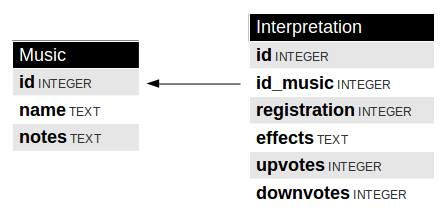
\includegraphics[width=\textwidth]{images/tree.jpg}
\caption{Árvore da base de dados, com as tabelas da música (\emph{musics}) e interpretação (\emph{interpretation}).}
\label{tree}
\end{figure}